\documentclass[slidestop]{beamer}
\usepackage{beamerthemesplit}
\usepackage{graphics}
\usepackage{pstricks}

\title{Simple-V RISC-V Extension for Vectorisation and SIMD}
\author{Luke Kenneth Casson Leighton}


\begin{document}

\frame{
   \begin{center}
    \huge{Simple-V RISC-V Parallelism Abstraction Extension}\\
    \vspace{32pt}
    \Large{Flexible Vectorisation}\\
    \Large{(aka not so Simple-V?)}\\
    \Large{(aka A Parallelism API for the RISC-V ISA)}\\
    \vspace{24pt}
    \Large{[proposed for] Chennai 9th RISC-V Workshop}\\
    \vspace{16pt}
    \large{\today}
  \end{center}
}


\frame{\frametitle{Credits and Acknowledgements}

 \begin{itemize}
   \item The Designers of RISC-V\vspace{15pt}
   \item The RVV Working Group and contributors\vspace{15pt}
   \item Allen Baum, Jacob Bachmeyer, Xan Phung, Chuanhua Chang,\\
	     Guy Lemurieux, Jonathan Neuschafer, Roger Brussee,
	     and others\vspace{15pt}
   \item ISA-Dev Group Members\vspace{10pt}
  \end{itemize}
}


\frame{\frametitle{Quick refresher on SIMD}

 \begin{itemize}
   \item SIMD very easy to implement (and very seductive)\vspace{8pt}
   \item Parallelism is in the ALU\vspace{8pt}
   \item Zero-to-Negligeable impact for rest of core\vspace{8pt}
  \end{itemize}
  Where SIMD Goes Wrong:\vspace{10pt}
   \begin{itemize}
   \item See "SIMD instructions considered harmful"
   https://sigarch.org/simd-instructions-considered-harmful
   \item Setup and corner-cases alone are extremely complex.\\
	     Hardware is easy, but software is hell.
   \item O($N^{6}$) ISA opcode proliferation!\\
	     opcode, elwidth, veclen, src1-src2-dest hi/lo
  \end{itemize}
}

\frame{\frametitle{Quick refresher on RVV}

 \begin{itemize}
   \item Effectively a variant of SIMD / SIMT (arbitrary length)\vspace{4pt}
   \item Extremely powerful (extensible to 256 registers)\vspace{4pt}
   \item Supports polymorphism, several datatypes (inc. FP16)\vspace{4pt}
   \item Requires a separate Register File (32 w/ext to 256)\vspace{4pt}
   \item Implemented as a separate pipeline (no impact on scalar)
  \end{itemize}
  However...
   \begin{itemize}
   \item 98 percent opcode duplication with rest of RV (CLIP)
   \item Extending RVV requires customisation not just of h/w:\\
	     gcc, binutils also need customisation (and maintenance)
   \item Fascinatingly, despite being a SIMD-variant, RVV only has
         O(N) opcode proliferation! (extremely well designed)
  \end{itemize}
}


\frame{\frametitle{The Simon Sinek lowdown (Why, How, What)}

 \begin{itemize}
   \item Why?
         Implementors need flexibility in vectorisation to optimise for
         area or performance depending on the scope:
	     embedded DSP, Mobile GPU's, Server CPU's and more.\\
		 Compilers also need flexibility in vectorisation to optimise for cost 
		 of pipeline setup, amount of state to context switch
		 and software portability
   \item How?
	     By marking INT/FP regs as "Vectorised" and
	     adding a level of indirection,
	     SV expresses how existing instructions should act 
	     on [contiguous] blocks of registers, in parallel, WITHOUT
	     needing any new extra arithmetic opcodes.
   \item What?
		 Simple-V is an "API" that implicitly extends
		 existing (scalar) instructions with explicit parallelisation\\
		 i.e. SV is actually about parallelism NOT vectors per se.\\
		 Has a lot in common with VLIW (without the actual VLIW).
  \end{itemize}
}


\frame{\frametitle{What's the value of SV? Why adopt it even in non-V?}

 \begin{itemize}
   \item memcpy becomes much smaller (higher bang-per-buck)
   \item context-switch (LOAD/STORE multiple): 1-2 instructions
   \item Compressed instrs further reduces I-cache (etc.)
   \item Reduced I-cache load (and less I-reads)
   \item Amazingly, SIMD becomes tolerable (no corner-cases)
   \item Modularity/Abstraction in both the h/w and the toolchain.
   \item "Reach" of registers accessible by Compressed is enhanced
   \item Future: double the standard INT/FP register file sizes.
  \end{itemize}
  Note:
   \begin{itemize}
   \item It's not just about Vectors: it's about instruction effectiveness
   \item Anything implementor is not interested in HW-optimising,\\
	     let it fall through to exceptions (implement as a trap).
  \end{itemize}
}


\frame{\frametitle{How does Simple-V relate to RVV? What's different?}

 \begin{itemize}
   \item RVV very heavy-duty (excellent for supercomputing)\vspace{8pt}
   \item Simple-V abstracts parallelism (based on best of RVV)\vspace{8pt}
   \item Graded levels: hardware, hybrid or traps (fit impl. need)\vspace{8pt}
   \item Even Compressed become vectorised (RVV can't)\vspace{8pt}
   \item No polymorphism in SV (too complex)\vspace{8pt}
  \end{itemize}
  What Simple-V is not:\vspace{4pt}
   \begin{itemize}
   \item A full supercomputer-level Vector Proposal
   \item A replacement for RVV (SV is designed to be over-ridden\\
	     by - or augmented to become - RVV)
  \end{itemize}
}


\frame{\frametitle{How is Parallelism abstracted in Simple-V?}

 \begin{itemize}
   \item Register "typing" turns any op into an implicit Vector op:\\
         registers are reinterpreted through a level of indirection
   \item Primarily at the Instruction issue phase (except SIMD)\\
         Note: it's ok to pass predication through to ALU (like SIMD)
   \item Standard and future and custom opcodes now parallel\\
         (crucially: with NO extra instructions needing to be added)
  \end{itemize}
  Note: EVERYTHING is parallelised:
   \begin{itemize}
   \item All LOAD/STORE (inc. Compressed, Int/FP versions)
   \item All ALU ops (Int, FP, SIMD, DSP, everything)
   \item All branches become predication targets (C.FNE added?)
   \item C.MV of particular interest (s/v, v/v, v/s)
   \item FCVT, FMV, FSGNJ etc. very similar to C.MV
  \end{itemize}
}


\frame{\frametitle{What's the deal / juice / score?}

 \begin{itemize}
   \item Standard Register File(s) overloaded with CSR "reg is vector"\\
	     (see pseudocode slides for examples)
   \item "2nd FP\&INT register bank" possibility, reserved for future\\
         (would allow standard regfiles to remain unmodified)
   \item Element width concept remain same as RVV\\
	     (CSRs give new size: overrides opcode-defined meaning)
   \item CSRs are key-value tables (overlaps allowed: v. important)
  \end{itemize}
  Key differences from RVV:
   \begin{itemize}
   \item Predication in INT reg as a BIT field (max VL=XLEN)
   \item Minimum VL must be Num Regs - 1 (all regs single LD/ST)
   \item SV may condense sparse Vecs: RVV cannot (SIMD-like):\\
         SV gives choice to Zero or skip non-predicated elements\\
         (no such choice in RVV: zeroing-only)
  \end{itemize}
}


\begin{frame}[fragile]
\frametitle{ADD pseudocode (or trap, or actual hardware loop)}

\begin{semiverbatim}
function op\_add(rd, rs1, rs2, predr) # add not VADD!
  int i, id=0, irs1=0, irs2=0;
  for (i = 0; i < VL; i++)
    if (ireg[predr] & 1<<i) # predication uses intregs
       ireg[rd+id] <= ireg[rs1+irs1] + ireg[rs2+irs2];
    if (reg\_is\_vectorised[rd] )  \{ id += 1; \}
    if (reg\_is\_vectorised[rs1])  \{ irs1 += 1; \}
    if (reg\_is\_vectorised[rs2])  \{ irs2 += 1; \}
\end{semiverbatim}

  \begin{itemize}
   \item Above is oversimplified: Reg. indirection left out (for clarity).
   \item SIMD slightly more complex (case above is elwidth = default)
   \item Scalar-scalar and scalar-vector and vector-vector now all in one
   \item OoO may choose to push ADDs into instr. queue (v. busy!)
  \end{itemize}
\end{frame}

% yes it really *is* ADD not VADD.  that's the entire point of
% this proposal, that *standard* operations are overloaded to
% become vectorised-on-demand


\begin{frame}[fragile]
\frametitle{Predication-Branch (or trap, or actual hardware loop)}

\begin{semiverbatim}
s1 = reg\_is\_vectorised(src1);
s2 = reg\_is\_vectorised(src2);
if (!s2 && !s1) goto branch;
for (int i = 0; i < VL; ++i)
  if (cmp(s1 ? reg[src1+i]:reg[src1],
          s2 ? reg[src2+i]:reg[src2])
         ireg[rs3] |= 1<<i;
\end{semiverbatim}

  \begin{itemize}
   \item SIMD slightly more complex (case above is elwidth = default)  
   \item If s1 and s2 both scalars, Standard branch occurs
   \item Predication stored in integer regfile as a bitfield
   \item Scalar-vector and vector-vector supported
   \item Overload Branch immediate to be predication target rs3
  \end{itemize}
\end{frame}

\begin{frame}[fragile]
\frametitle{VLD/VLD.S/VLD.X (or trap, or actual hardware loop)}

\begin{semiverbatim}
if (unit-strided) stride = elsize;
else stride = areg[as2]; // constant-strided
for (int i = 0; i < VL; ++i)
  if ([!]preg[rd] & 1<<i)
    for (int j = 0; j < seglen+1; j++)
      if (reg\_is\_vectorised[rs2]) offs = vreg[rs2+i]
      else offs = i*(seglen+1)*stride;
      vreg[rd+j][i] = mem[sreg[base] + offs + j*stride]
\end{semiverbatim}

  \begin{itemize}
   \item Again: elwidth != default slightly more complex
   \item rs2 vectorised taken to implicitly indicate VLD.X
  \end{itemize}
\end{frame}


\frame{\frametitle{Register key-value CSR store (lookup table / CAM)}

 \begin{itemize}
   \item key is int regfile number or FP regfile number (1 bit)
   \item treated as vector if referred to in op (5 bits, key)
   \item starting register to actually be used (5 bits, value)
   \item element bitwidth: default, dflt/2, 8, 16 (2 bits)
   \item is vector: Y/N (1 bit)
   \item is packed SIMD: Y/N (1 bit)
   \item register bank: 0/reserved for future ext. (1 bit)
  \end{itemize}
  Notes:
   \begin{itemize}
   \item References different (internal) mapping table for INT or FP
   \item Level of indirection has implications for pipeline latency
   \item (future) bank bit, no need to extend opcodes: set bank=1,
         just use normal 5-bit regs, indirection takes care of the rest.
  \end{itemize}
}


\frame{\frametitle{Register element width and packed SIMD}

  Packed SIMD = N:
 \begin{itemize}
   \item default: RV32/64/128 opcodes define elwidth = 32/64/128
   \item default/2: RV32/64/128 opcodes, elwidth = 16/32/64 with
         top half of register ignored (src), zero'd/s-ext (dest)
   \item 8 or 16: elwidth = 8 (or 16), similar to default/2
  \end{itemize}
  Packed SIMD = Y (default is moot, packing is 1:1)
 \begin{itemize}
   \item default/2: 2 elements per register @ opcode-defined bitwidth
   \item 8 or 16: standard 8 (or 16) packed SIMD
  \end{itemize}
  Notes:
 \begin{itemize}
   \item Different src/dest widths (and packs) PERMITTED
   \item RV* already allows (and defines) how RV32 ops work in RV64\\
         so just logically follow that lead/example.
  \end{itemize}
}


\begin{frame}[fragile]
\frametitle{Register key-value CSR table decoding pseudocode}

\begin{semiverbatim}
struct vectorised fp\_vec[32], int\_vec[32]; // 64 in future
for (i = 0; i < 16; i++) // 16 CSRs?
   tb = int\_vec if CSRvec[i].type == 0 else fp\_vec
   idx = CSRvec[i].regkey // INT/FP src/dst reg in opcode
   tb[idx].elwidth  = CSRvec[i].elwidth
   tb[idx].regidx   = CSRvec[i].regidx  // indirection
   tb[idx].isvector = CSRvec[i].isvector
   tb[idx].packed   = CSRvec[i].packed  // SIMD or not
   tb[idx].bank     = CSRvec[i].bank    // 0 (1=rsvd)
   tb[idx].enabled  = true
\end{semiverbatim}

 \begin{itemize}
   \item All 32 int (and 32 FP) entries zero'd before setup
   \item Might be a bit complex to set up in hardware (keep as CAM?)
  \end{itemize}

\end{frame}


\frame{\frametitle{Predication key-value CSR store}

 \begin{itemize}
   \item key is int regfile number or FP regfile number (1 bit)
   \item register to be predicated if referred to (5 bits, key)
   \item INT reg with actual predication mask (5 bits, value)
   \item predication is inverted Y/N (1 bit)
   \item non-predicated elements are to be zero'd Y/N (1 bit)
   \item register bank: 0/reserved for future ext. (1 bit)
  \end{itemize}
  Notes:\vspace{10pt}
   \begin{itemize}
   \item Table should be expanded out for high-speed implementations
   \item Key-value overlaps permitted, but (key+type) must be unique
   \item RVV rules about deleting higher-indexed CSRs followed
  \end{itemize}
}


\begin{frame}[fragile]
\frametitle{Predication key-value CSR table decoding pseudocode}

\begin{semiverbatim}
struct pred fp\_pred[32], int\_pred[32]; // 64 in future
for (i = 0; i < 16; i++) // 16 CSRs?
   tb = int\_pred if CSRpred[i].type == 0 else fp\_pred
   idx = CSRpred[i].regkey
   tb[idx].zero     = CSRpred[i].zero    // zeroing
   tb[idx].inv      = CSRpred[i].inv     // inverted
   tb[idx].predidx  = CSRpred[i].predidx // actual reg
   tb[idx].bank     = CSRpred[i].bank    // 0 for now
   tb[idx].enabled  = true
\end{semiverbatim}

 \begin{itemize}
   \item All 32 int and 32 FP entries zero'd before setting\\
	     (predication disabled)
   \item Might be a bit complex to set up in hardware (keep as CAM?)
  \end{itemize}

\end{frame}


\begin{frame}[fragile]
\frametitle{Get Predication value pseudocode}

\begin{semiverbatim}
def get\_pred\_val(bool is\_fp\_op, int reg):
   tb = int\_pred if is\_fp\_op else fp\_pred
   if (!tb[reg].enabled):
      return ~0x0              // all ops enabled
   predidx = tb[reg].predidx   // redirection occurs HERE
   predicate = intreg[predidx] // actual predicate HERE
   if (tb[reg].inv):
      predicate = ~predicate   // invert ALL bits
   return predicate
\end{semiverbatim}

 \begin{itemize}
   \item References different (internal) mapping table for INT or FP
   \item Actual predicate bitmask ALWAYS from the INT regfile
   \item Hard-limit on MVL of XLEN (predication only 1 intreg)
  \end{itemize}

\end{frame}


\frame{\frametitle{To Zero or not to place zeros in non-predicated elements?}

 \begin{itemize}
   \item Zeroing is an implementation optimisation favouring OoO
   \item Simple implementations may skip non-predicated operations
   \item Simple implementations explicitly have to destroy data
   \item Complex implementations may use reg-renames to save power\\
	     Zeroing on predication chains makes optimisation harder
   \item Compromise: REQUIRE both (specified in predication CSRs).
  \end{itemize}
  Considerations:
  \begin{itemize}
   \item Complex not really impacted, simple impacted a LOT\\
         with Zeroing... however it's useful (memzero)
   \item Non-zero'd overlapping "Vectors" may issue overlapping ops\\
	     (2nd op's predicated elements slot in 1st's non-predicated ops)
   \item Please don't use Vectors for "security" (use Sec-Ext)
  \end{itemize}
}
% with overlapping "vectors" - bearing in mind that "vectors" are
% just a remap onto the standard register file, if the top bits of
% predication are zero, and there happens to be a second vector
% that uses some of the same register file that happens to be
% predicated out, the second vector op may be issued *at the same time*
% if there are available parallel ALUs to do so.


\frame{\frametitle{Implementation Options}

 \begin{itemize}
   \item Absolute minimum: Exceptions: if CSRs indicate "V", trap.\\
         (Requires as absolute minimum that CSRs be in Hardware)
   \item Hardware loop, single-instruction issue\\
		 (Do / Don't send through predication to ALU)
   \item Hardware loop, parallel (multi-instruction) issue\\
         (Do / Don't send through predication to ALU)
   \item Hardware loop, full parallel ALU (not recommended)
  \end{itemize}
  Notes:\vspace{4pt}
  \begin{itemize}
   \item 4 (or more?) options above may be deployed on per-op basis
   \item SIMD always sends predication bits to ALU (if requested)
   \item Minimum MVL MUST be sufficient to cover regfile LD/ST
   \item Instr. FIFO may repeatedly split off N scalar ops at a time
  \end{itemize}
}
% Instr. FIFO may need its own slide.  Basically, the vectorised op
% gets pushed into the FIFO, where it is then "processed".  Processing
% will remove the first set of ops from its vector numbering (taking
% predication into account) and shoving them **BACK** into the FIFO,
% but MODIFYING the remaining "vectorised" op, subtracting the now
% scalar ops from it.

\frame{\frametitle{Predicated 8-parallel ADD: 1-wide ALU (no zeroing)}
 \begin{center}
  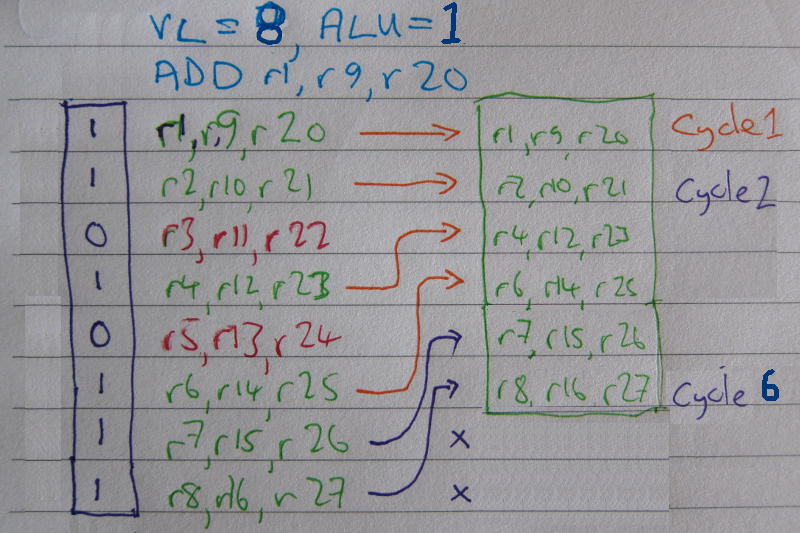
\includegraphics[height=2.5in]{padd9_alu1.png}\\
  {\bf \red Predicated adds are shuffled down: 6 cycles in total}
 \end{center}
}


\frame{\frametitle{Predicated 8-parallel ADD: 4-wide ALU (no zeroing)}
 \begin{center}
  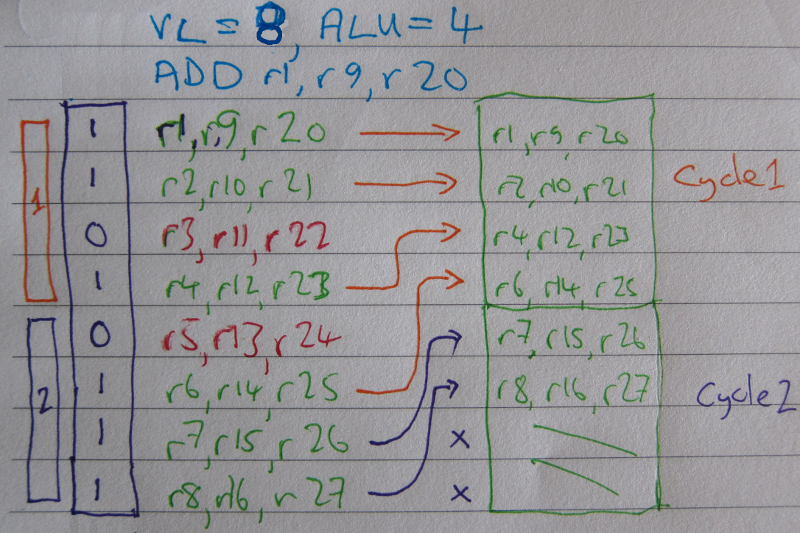
\includegraphics[height=2.5in]{padd9_alu4.png}\\
  {\bf \red Predicated adds are shuffled down: 4 in 1st cycle, 2 in 2nd}
 \end{center}
}


\frame{\frametitle{Predicated 8-parallel ADD: 3 phase FIFO expansion}
 \begin{center}
  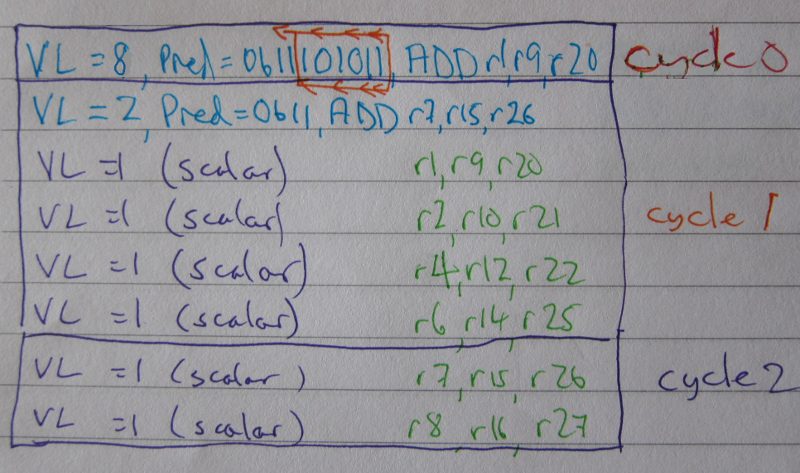
\includegraphics[height=2.5in]{padd9_fifo.png}\\
  {\bf \red First cycle takes first four 1s; second takes the rest}
 \end{center}
}


\begin{frame}[fragile]
\frametitle{ADD pseudocode with redirection (and proper predication)}

\begin{semiverbatim}
function op\_add(rd, rs1, rs2) # add not VADD!
  int i, id=0, irs1=0, irs2=0;
  rd  = int\_vec[rd ].isvector ? int\_vec[rd ].regidx : rd;
  rs1 = int\_vec[rs1].isvector ? int\_vec[rs1].regidx : rs1;
  rs2 = int\_vec[rs2].isvector ? int\_vec[rs2].regidx : rs2;
  predval = get\_pred\_val(FALSE, rd);
  for (i = 0; i < VL; i++)
    if (predval \& 1<<i) # predication uses intregs
       ireg[rd+id] <= ireg[rs1+irs1] + ireg[rs2+irs2];
    if (int\_vec[rd ].isvector)  \{ id += 1; \}
    if (int\_vec[rs1].isvector)  \{ irs1 += 1; \}
    if (int\_vec[rs2].isvector)  \{ irs2 += 1; \}
\end{semiverbatim}

  \begin{itemize}
   \item SIMD (elwidth != default) not covered above
  \end{itemize}
\end{frame}


\frame{\frametitle{How are SIMD Instructions Vectorised?}

 \begin{itemize}
   \item SIMD ALU(s) primarily unchanged
   \item Predication added down to each SIMD element (if requested,
         otherwise entire block will be predicated as a whole)
   \item Predication bits sent in groups to the ALU (if requested,
         otherwise just one bit for the entire packed block)
   \item End of Vector enables (additional) predication:
	     completely nullifies end-case code (ONLY in multi-bit
	     predication mode)
  \end{itemize}
  Considerations:
   \begin{itemize}
   \item Many SIMD ALUs possible (parallel execution)
   \item Implementor free to choose (API remains the same)
   \item Unused ALU units wasted, but s/w DRASTICALLY simpler
   \item Very long SIMD ALUs could waste significant die area
  \end{itemize}
}
% With multiple SIMD ALUs at for example 32-bit wide they can be used
% to either issue 64-bit or 128-bit or 256-bit wide SIMD operations
% or they can be used to cover several operations on totally different
% vectors / registers.

\frame{\frametitle{Predicated 9-parallel SIMD ADD (Packed=Y)}
 \begin{center}
  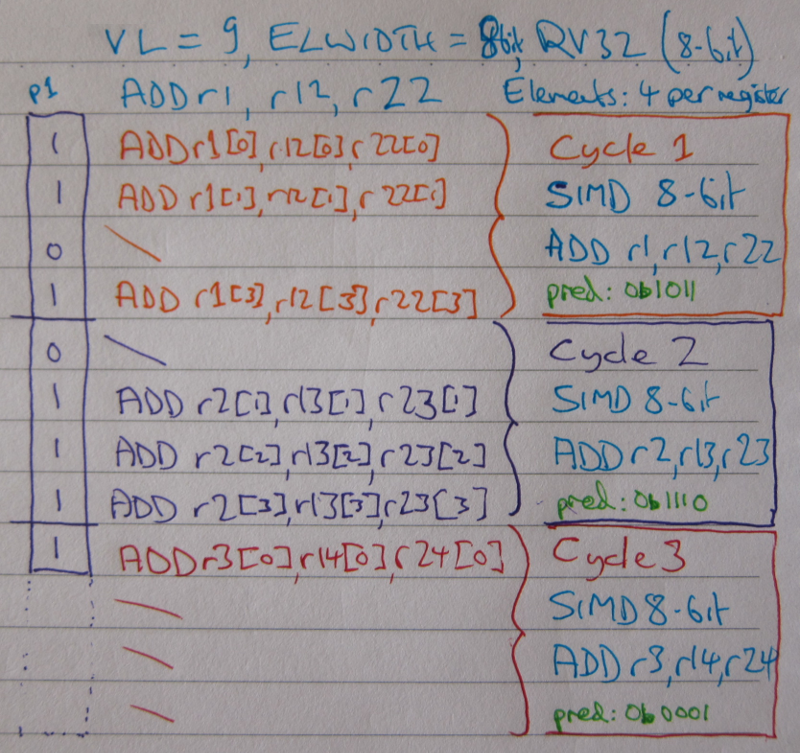
\includegraphics[height=2.5in]{padd9_simd.png}\\
  {\bf \red 4-wide 8-bit SIMD, 4 bits of predicate passed to ALU}
 \end{center}
}


\frame{\frametitle{Why are overlaps allowed in Regfiles?}

 \begin{itemize}
   \item Same target register(s) can have multiple "interpretations"
   \item CSRs are costly to write to (do it once)
   \item Set "real" register (scalar) without needing to set/unset CSRs.
   \item xBitManip plus SIMD plus xBitManip = Hi/Lo bitops
   \item (32-bit GREV plus 4x8-bit SIMD plus 32-bit GREV:\\
	     GREV @ VL=N,wid=32; SIMD @ VL=Nx4,wid=8)
   \item RGB 565 (video): BEXTW plus 4x8-bit SIMD plus BDEPW\\
	     (BEXT/BDEP @ VL=N,wid=32; SIMD @ VL=Nx4,wid=8)
   \item Same register(s) can be offset (no need for VSLIDE)\vspace{6pt}
  \end{itemize}
  Note:
   \begin{itemize}
   \item xBitManip reduces O($N^{6}$) SIMD down to O($N^{3}$) on its own.
   \item Hi-Performance: Macro-op fusion (more pipeline stages?)
  \end{itemize}
}


\frame{\frametitle{C.MV extremely flexible!}

 \begin{itemize}
   \item scalar-to-vector (w/ no pred): VSPLAT
   \item scalar-to-vector (w/ dest-pred): Sparse VSPLAT
   \item scalar-to-vector (w/ 1-bit dest-pred): VINSERT
   \item vector-to-scalar (w/ [1-bit?] src-pred): VEXTRACT
   \item vector-to-vector (w/ no pred): Vector Copy
   \item vector-to-vector (w/ src pred): Vector Gather (inc VSLIDE)
   \item vector-to-vector (w/ dest pred): Vector Scatter (inc. VSLIDE)
   \item vector-to-vector (w/ src \& dest pred): Vector Gather/Scatter
  \end{itemize}
  \vspace{4pt}
  Notes:
   \begin{itemize}
   \item Surprisingly powerful! Zero-predication even more so
   \item Same arrangement for FCVT, FMV, FSGNJ etc.
  \end{itemize}
}


\begin{frame}[fragile]
\frametitle{MV pseudocode with predication}

\begin{semiverbatim}
function op\_mv(rd, rs) # MV not VMV!
  rd = int\_vec[rd].isvector ? int\_vec[rd].regidx : rd;
  rs = int\_vec[rs].isvector ? int\_vec[rs].regidx : rs;
  ps = get\_pred\_val(FALSE, rs); # predication on src
  pd = get\_pred\_val(FALSE, rd); # ... AND on dest
  for (int i = 0, int j = 0; i < VL && j < VL;):
    if (int\_vec[rs].isvec) while (!(ps \& 1<<i)) i++;
    if (int\_vec[rd].isvec) while (!(pd \& 1<<j)) j++;
    ireg[rd+j] <= ireg[rs+i];
    if (int\_vec[rs].isvec) i++;
    if (int\_vec[rd].isvec) j++;
\end{semiverbatim}

  \begin{itemize}
   \item elwidth != default not covered above (might be a bit hairy)
   \item Ending early with 1-bit predication not included (VINSERT)
  \end{itemize}
\end{frame}


\begin{frame}[fragile]
\frametitle{VSELECT: stays or goes? Stays if MV.X exists...}

\begin{semiverbatim}
def op_mv_x(rd, rs):         # (hypothetical) RV MX.X
   rs = regfile[rs]          # level of indirection (MV.X)
   regfile[rd] = regfile[rs] # straight regcopy
\end{semiverbatim}

Vectorised version aka "VSELECT":

\begin{semiverbatim}
def op_mv_x(rd, rs):              # SV version of MX.X
   for i in range(VL):
      rs1 = regfile[rs+i]         # indirection
      regfile[rd+i] = regfile[rs] # straight regcopy
\end{semiverbatim}

  \begin{itemize}
   \item However MV.X does not exist in RV, so neither can VSELECT
   \item \red SV is not about adding new functionality, only parallelism
  \end{itemize}


\end{frame}


\frame{\frametitle{Opcodes, compared to RVV}

 \begin{itemize}
   \item All integer and FP opcodes all removed (no CLIP, FNE)
   \item VMPOP, VFIRST etc. all removed (use xBitManip)
   \item VSLIDE removed (use regfile overlaps)
   \item C.MV covers VEXTRACT VINSERT and VSPLAT (and more)
   \item Vector (or scalar-vector) copy: use C.MV (MV is a pseudo-op)
   \item VMERGE: twin predicated C.MVs (one inverted. macro-op'd)
   \item VSETVL, VGETVL stay (the only ops that do!)
  \end{itemize}
  Issues:
 \begin{itemize}
   \item VSELECT stays? no MV.X, so no (add with custom ext?)
   \item VSNE exists, but no FNE (use predication inversion?)
   \item VCLIP is not in RV* (add with custom ext? or CSR?)
  \end{itemize}
}


\begin{frame}[fragile]
\frametitle{Example c code: DAXPY}

\begin{semiverbatim}
    void daxpy(size_t n, double a,
               const double x[], double y[])
    \{
     for (size_t i = 0; i < n; i++) \{
       y[i] = a*x[i] + y[i];
     \}
    \}
\end{semiverbatim}

  \begin{itemize}
   \item See "SIMD Considered Harmful" for SIMD/RVV analysis\\
	   https://sigarch.org/simd-instructions-considered-harmful/
  \end{itemize}


\end{frame}


\begin{frame}[fragile]
\frametitle{RVV DAXPY assembly (RV32V)}

\begin{semiverbatim}
# a0 is n, a1 is ptr to x[0], a2 is ptr to y[0], fa0 is a
 li t0, 2<<25
 vsetdcfg t0            # enable 2 64b Fl.Pt. registers
loop:
 setvl  t0, a0          # vl = t0 = min(mvl, n)
 vld    v0, a1          # load vector x
 slli   t1, t0, 3       # t1 = vl * 8 (in bytes)
 vld    v1, a2          # load vector y
 add    a1, a1, t1      # increment pointer to x by vl*8
 vfmadd v1, v0, fa0, v1 # v1 += v0 * fa0 (y = a * x + y)
 sub    a0, a0, t0      # n -= vl (t0)
 vst    v1, a2          # store Y
 add    a2, a2, t1      # increment pointer to y by vl*8
 bnez   a0, loop        # repeat if n != 0
\end{semiverbatim}
\end{frame}


\begin{frame}[fragile]
\frametitle{SV DAXPY assembly (RV64D)}

\begin{semiverbatim}
# a0 is n, a1 is ptr to x[0], a2 is ptr to y[0], fa0 is a
 CSRvect1 = \{type: F, key: a3, val: a3, elwidth: dflt\}
 CSRvect2 = \{type: F, key: a7, val: a7, elwidth: dflt\}
loop:
 setvl  t0, a0, 4       # vl = t0 = min(min(mvl, 4, n))
 ld     a3, a1          # load 4 registers a3-6 from x
 slli   t1, t0, 3       # t1 = vl * 8 (in bytes)
 ld     a7, a2          # load 4 registers a7-10 from y
 add    a1, a1, t1      # increment pointer to x by vl*8
 fmadd  a7, a3, fa0, a7 # v1 += v0 * fa0 (y = a * x + y)
 sub    a0, a0, t0      # n -= vl (t0)
 st     a7, a2          # store 4 registers a7-10 to y
 add    a2, a2, t1      # increment pointer to y by vl*8
 bnez   a0, loop        # repeat if n != 0
\end{semiverbatim}
\end{frame}


\frame{\frametitle{Under consideration (some answers documented)}

 \begin{itemize}
   \item Should future extra bank be included now?
   \item How many Register and Predication CSRs should there be?\\
         (and how many in RV32E)
   \item How many in M-Mode (for doing context-switch)?
   \item Should use of registers be allowed to "wrap" (x30 x31 x1 x2)?
   \item Can CLIP be done as a CSR (mode, like elwidth)
   \item SIMD saturation (etc.) also set as a mode?
   \item Include src1/src2 predication on Comparison Ops?\\
	     (same arrangement as C.MV, with same flexibility/power)
   \item 8/16-bit ops is it worthwhile adding a "start offset"? \\
         (a bit like misaligned addressing... for registers)\\
         or just use predication to skip start?
   \item see http://libre-riscv.org/simple\_v\_extension/\#issues
  \end{itemize}
}


\frame{\frametitle{What's the downside(s) of SV?}
 \begin{itemize}
   \item EVERY register operation is inherently parallelised\\
	     (scalar ops are just vectors of length 1)\vspace{4pt}
   \item Tightly coupled with the core (instruction issue)\\
         could be disabled through MISA switch\vspace{4pt}
   \item An extra pipeline phase almost certainly essential\\
         for fast low-latency implementations\vspace{4pt}
   \item With zeroing off, skipping non-predicated elements is hard:\\
         it is however an optimisation (and need not be done).\vspace{4pt}
   \item Setting up the Register/Predication tables (interpreting the\\
	     CSR key-value stores) might be a bit complex to optimise
	     (any change to a CSR key-value entry needs to redo the table)
  \end{itemize}
}


\frame{\frametitle{Summary}

 \begin{itemize}
   \item Actually about parallelism, not Vectors (or SIMD) per se\\
         and NOT about adding new ALU/logic/functionality.
   \item Only needs 2 actual instructions (plus the CSRs).\\
         RVV - and "standard" SIMD - require ISA duplication
   \item Designed for flexibility (graded levels of complexity)
   \item Huge range of implementor freedom
   \item Fits RISC-V ethos: achieve more with less
   \item Reduces SIMD ISA proliferation by 3-4 orders of magnitude \\
	     (without SIMD downsides or sacrificing speed trade-off)
   \item Covers 98\% of RVV, allows RVV to fit "on top"
   \item Byproduct of SV is a reduction in code size, power usage
	     etc. (increase efficiency, just like Compressed)
  \end{itemize}
}


\frame{
  \begin{center}
    {\Huge The end\vspace{20pt}\\
		   Thank you\vspace{20pt}\\
		   Questions?\vspace{20pt}
	}
  \end{center}
  
  \begin{itemize}
	\item Discussion: ISA-DEV mailing list
	\item http://libre-riscv.org/simple\_v\_extension/
  \end{itemize}
}


\end{document}
